\documentclass{article}  
\usepackage{graphicx}
\usepackage{subfig}
\usepackage{hyperref}
\usepackage{amsmath}
\usepackage{amssymb}
\usepackage{gensymb}
\begin{document}  




\title{Simple Pendulum}

\author{Yogesh Swami}
\maketitle
 
 
 
\begin{abstract}
In this report, I have worked on the non-linear equation of motion of the simple pendulum. First, I will derive the equation of motion of simple pendulum. Then I will talk about its non-linearity and how it can be linearized. After this theory, this report will present angle(rad) vs time(s) plot using python code.
\end{abstract}


\section{Introduction}
\paragraph{}The simple pendulum is formed of a light, stiff, inextensible rod of length l with a bob of mass m. Its position with respect to time t can be described merely by the angle $\theta$ (measured against a reference line, usually taken as the vertical line straight down). The fact that its position can be described by using only one variable means that the simple pendulum has only one degree of freedom.
\paragraph{}
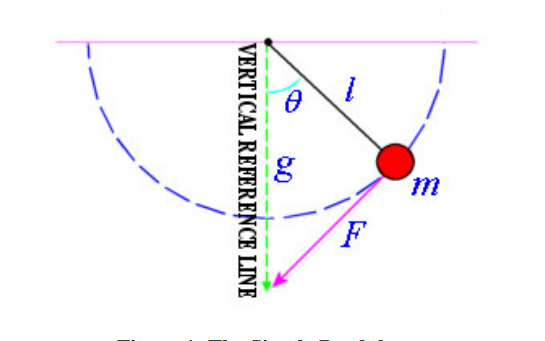
\includegraphics[width=65mm]{pendulum.png}
\paragraph{}From Figure, it can be seen that the driving force of the pendulum is: \begin{center}
F = −mg sin($\theta$)
\end{center}
\paragraph{}Remember that the acceleration g is moving downwards, hence the negative sign.Now if we take the displacement of the bob from its equilibrium state (hanging exactly straight up or down) to be s, then the acceleration of the bob is $\ddot{s}$.
\paragraph{}Newton’s second law of motion states that: F = ma
\paragraph{}Where F denotes a force, m denotes a mass, and a denotes acceleration.
\paragraph{}So therefore: \begin{center}
-mgsin($\theta$) = m$\ddot{s}$ \\ -gsin($\theta$) = $\ddot{s}$
\end{center}
\paragraph{}And when the rod makes an angle $\theta$ with the vertical, then the displacement s of the bob is
given by:\begin{center}
s = l$\theta$
\end{center}
\paragraph{}Differentiating this twice with respect to time t gives us:\begin{center}
$\ddot{s}$ = l$\ddot{\theta}$
\end{center}
\paragraph{}Substituting this into (1) and rearranging:\begin{center}
l$\ddot{\theta}$ = -gsin($\theta$)
\end{center}
\paragraph{}Thus,\begin{center}
$\ddot{\theta}$ = -$\dfrac{g}{l}$sin($\theta$)
\end{center}
\paragraph{} This is the non-linear equation of motion of simple pendulum.



\section{Talking about Equation}
Now as we have derived non-linear equation of motion of simple pendulum, let's discuss about non-linearity of this equation:
\begin{center}$\ddot{\theta}$ = -$\dfrac{g}{l}$sin($\theta$)\end{center}
\paragraph{}So, this equation is non-linear but it can be linearized for smaller values of $\theta$.
\paragraph{}If $\theta$ is small, ($\theta$ less than 10\degree):
\begin{center}
sin($\theta$) $\approx$ $\theta$
\end{center}

\paragraph{}Therefore,
\begin{center}
$\ddot{\theta}$ + $\omega^2\theta$ = 0 \\  where ( $\omega^2$ = $\dfrac{g}{l}$)
\end{center}

\paragraph{}This equation resembles same as simple harmonic oscillator equation. So, solution of this equation can be written as:
\begin{center}
$\theta$(t) = C\textsubscript{1}cos($\omega$t) + C\textsubscript{2}sin($\omega$t)
\end{center}
\paragraph{}Initial conditions: Pendulum is raised to some angle $\theta$ which is zero initially.
\begin{center}
$\theta$(0) = $\theta$\textsubscript{0}
\\$\ddot{\theta}$(0) = 0  
\end{center}
\paragraph{}As velocity is zero at this point. So,
\begin{center}
$\ddot{\theta}$(0) = 0  
\end{center}
\paragraph{}If we substitute this into the solution, we find that :
\begin{center}
C\textsubscript{1} =  $\theta$\textsubscript{0}
\\C\textsubscript{2} = 0
\end{center}
\paragraph{}We can rewrite the solution as:
\begin{center}
$\theta$(t) = $\theta$\textsubscript{0}cos($\omega$t)
\end{center}
\paragraph{}Now talking about time period, as we know:
\begin{center}
$\omega$ = 2$\pi$f = $\dfrac{g}{l}$
\\ f = $\dfrac{1}{2\pi}\sqrt{\dfrac{g}{l}}$
\\ T = $\dfrac{1}{f}$
\\ T = 2$\pi\sqrt{\dfrac{l}{g}}$
\end{center}

\section{Numerical Solution to Simple Pendulum}
\paragraph{}We have this 2nd order ordinary differential equation:
\begin{center}
$\ddot{\theta}$ + $\dfrac{g}{l}$sin($\theta$) = 0
\\$\ddot{\theta}$ = -$\dfrac{g}{l}$sin($\theta$)
\end{center}
\paragraph{}In order to convert it into a 1st order differential equation, we define:
\begin{center}
X = $\ddot{\theta}$
\\ $\dot{X}$ = $\ddot{\theta}$
\\ $\dot{X}$ = -$\dfrac{g}{l}$sin($\theta$)
\end{center}

\paragraph{}Stacking above equations in matrix form,
\begin{center}
$$
\begin{bmatrix}
\dot{\theta} \\
\dot{X}
\end{bmatrix}
=
\begin{bmatrix}
X \\
-\dfrac{g}{l}sin(\theta)
\end{bmatrix}
$$
\end{center}

\paragraph{}Rewriting this in the form of :
\begin{center}
$\dot{\vec{Y}}$ = $\vec{F}$
\end{center}

\paragraph{}Writing this in discrete form :
\begin{center}
$\dfrac{\vec{Y}\textsubscript{t+1}-\vec{Y}\textsubscript{t}}{\Delta t}$ = $\vec{F}$
\end{center}

\paragraph{}So,
\begin{center}
$\vec{Y}$\textsubscript{t+1} = $\vec{Y}$\textsubscript{t} = $\Delta$t$\vec{F}$
\end{center}

\section{Plots}
\paragraph{}Here, I will show the different plots I got at different angles (0, 30, 60, 90, 120,150, 180).
\begin{figure}[h]
    \begin{minipage}{0.45\textwidth}
        \centering
        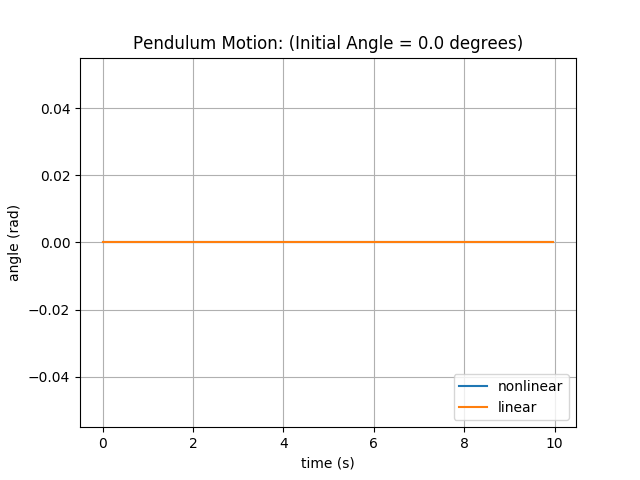
\includegraphics[width=1.2\textwidth]{Figure_0.png} % first figure itself
        \caption{0 degree}
    \end{minipage}\hfill
    \begin{minipage}{0.45\textwidth}
        \centering
        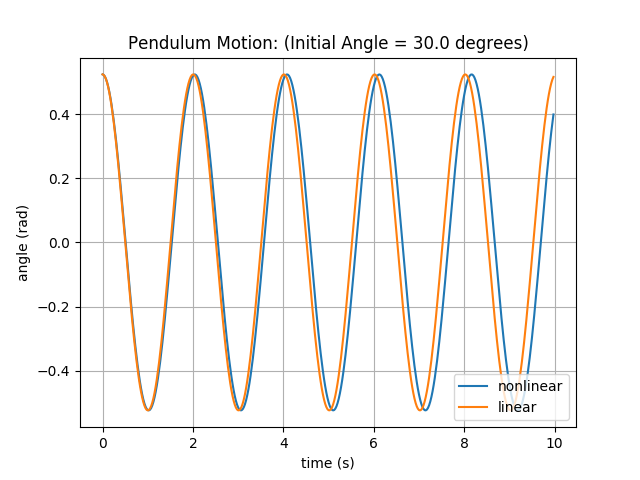
\includegraphics[width=1.2\textwidth]{Figure_30.png} % second figure itself
        \caption{30 degree}
    \end{minipage}
\end{figure}
\begin{figure}[h]
    \begin{minipage}{0.45\textwidth}
        \centering
        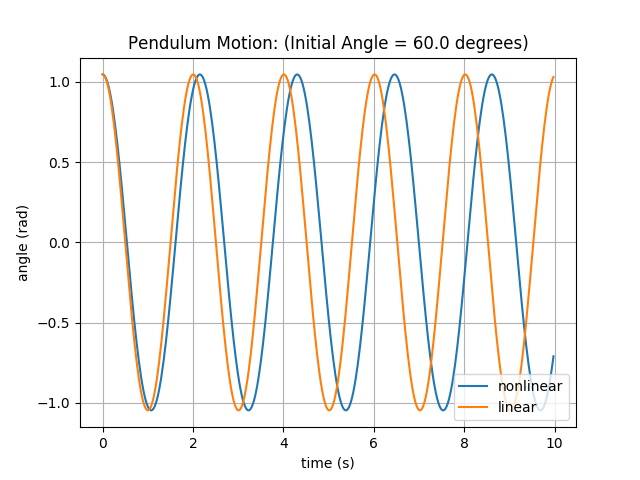
\includegraphics[width=1.2\textwidth]{Figure_60.png} % first figure itself
        \caption{60 degree}
    \end{minipage}\hfill
    \begin{minipage}{0.45\textwidth}
        \centering
        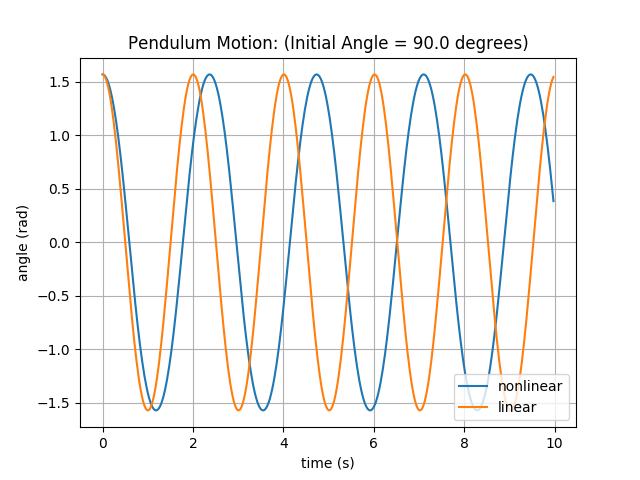
\includegraphics[width=1.2\textwidth]{Figure_90.png} % second figure itself
        \caption{90 degree}
    \end{minipage}
\end{figure}
\begin{figure}[h]
    \begin{minipage}{0.45\textwidth}
        \centering
        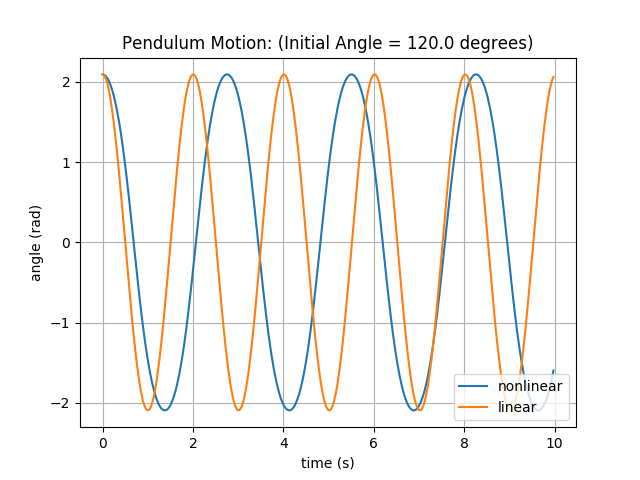
\includegraphics[width=1.2\textwidth]{Figure_120.png} % first figure itself
        \caption{120 degree}
    \end{minipage}\hfill
    \begin{minipage}{0.45\textwidth}
        \centering
        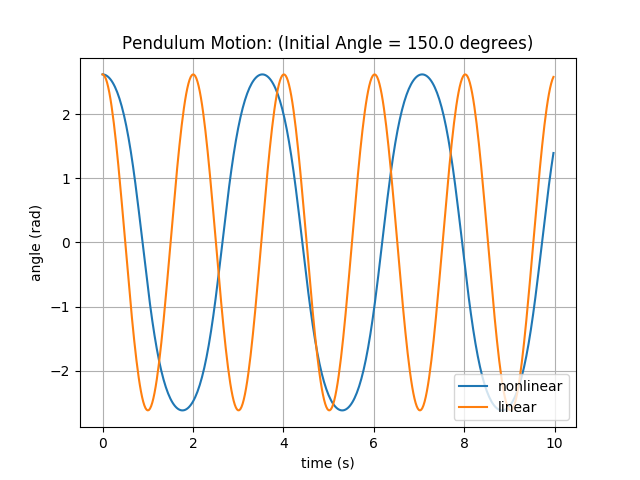
\includegraphics[width=1.2\textwidth]{Figure_150.png} % second figure itself
        \caption{150 degree}
    \end{minipage}
\end{figure}


\newpage
\section{Conclusion}
\paragraph{}So, we can conclude that  as angle increases from 0, its non-linearity increases. The period of the simple pendulum oscillations varies as square of the length of pendulum. The period of the simple pendulum oscillations does not depend on the mass of the load, nor on the angle of revolution.


\section{Acknowledgments}
\paragraph{}I would like to express my special thanks of gratitude to professor Anjan Kumar Giri who gave me the golden opportunity to do this wonderful project on non-linear dynamics, which also helped me in doing a lot of research and I came to know about so many new things.



\end{document}